\documentclass[9pt]{beamer}

\setbeamersize{text margin left=6mm,text margin right=8mm}

\usetheme[progressbar=frametitle]{metropolis}

% \usetheme[progressbar=frametitle]{Madrid}

\usepackage{xcolor}

\definecolor{bluegreen}{RGB}{3, 166, 155}
\definecolor{pitchblack}{RGB}{0, 0, 0}
\definecolor{lightbeige}{RGB}{255, 251, 241}
\definecolor{mediumgray}{RGB}{183, 183, 183}
\definecolor{mygreen}{rgb}{0,0.6,0}
\definecolor{mygray}{rgb}{0.5,0.5,0.5}
\definecolor{mymauve}{rgb}{0.58,0,0.82}
\definecolor{keywords}{RGB}{255,0,90}
\definecolor{comments}{RGB}{0,0,113}
\definecolor{red}{RGB}{160,0,0}
\definecolor{green}{RGB}{0,150,0}
\definecolor{navy}{RGB}{0,0,128}



% \setbeamercolor{progress bar}{fg=green,bg=blue}
% \setbeamercolor{background canvas}{bg=pitchblack}
% \setbeamercolor{normal text}{fg=lightbeige}
% \setbeamercolor{frametitle}{bg=bluegreen, fg=mediumgray}
\setbeamercolor{background canvas}{bg=white}
\setbeamercolor{normal text}{fg=black}
\setbeamercolor{frametitle}{bg=white, fg=black}



\usepackage{appendixnumberbeamer}
\usepackage{booktabs}
\usepackage[scale=2]{ccicons}

\usepackage{pgfplots}
\usepgfplotslibrary{dateplot}

\usepackage{xspace}
\newcommand{\themename}{\textbf{\textsc{metropolis}}\xspace}

\usepackage{fancyhdr}
\usepackage[mmddyyyy,hhmmss]{datetime}

% \date{\today}
\date{}
% \date[Last Compiled:]{\today}

\author{Kia Teymourian}
% \institute{ Slides last compiled: \today , Time: \currenttime}
% \institute{ Slides last compiled: \today}
\institute{June, 2019}


% This is important to set the default font to serif.
\usefonttheme{serif} % default family is serif

% \setmainfont{Liberation Serif}

% Packages for drawing arrows.
\usepackage{tikz}
\usepgflibrary{arrows}% for more options on arrows

\usepackage{pgfplots}
\usepgfplotslibrary{dateplot}
\usepackage{xspace}
% \newcommand{\themename}{\textbf{\textsc{metropolis}}\xspace}

\usepackage{blindtext}

\usepackage{listings}

% \usepackage{color}

\usepackage{caption}
\usepackage{graphicx}



\definecolor{backgroundCol}{rgb}{.97, .97, .97}
\definecolor{commentstyleCol}{rgb}{0, 0, 80}
\definecolor{keywordstyleCol}{rgb}{0.737,0.353,0.396}
\definecolor{stringstyleCol}{rgb}{0.192,0.494,0.8}
\definecolor{NumCol}{rgb}{0.686,0.059,0.569}
\definecolor{basicstyleCol}{rgb}{0.345, 0.345, 0.345}



\lstset{basicstyle=\ttfamily,
escapeinside={||},
mathescape=true}

\usepackage{algpseudocode}
\usepackage{MnSymbol,wasysym}

\definecolor{DarkGrenen}{RGB}{0,100,0}
\definecolor{DarkOliveGreen}{RGB}{85,107,47}

\definecolor{saddlebrown}{RGB}{139,69,19}




\newcommand{\red}[1]{\textcolor{red}{#1}}
\newcommand{\blue}[1]{\textcolor{blue}{#1}}
\newcommand{\green}[1]{\textcolor{DarkGrenen}{#1}}
\newcommand{\brown}[1]{\textcolor{saddlebrown}{#1}}


\newcommand{\redb}[1]{\textcolor{red}{\textbf{\boldmath{#1}}}}
\newcommand{\blueb}[1]{\textcolor{blue}{\textbf{\boldmath{#1}}}}
\newcommand{\greenb}[1]{\textcolor{DarkGrenen}{\textbf{\boldmath{#1}}}}
\newcommand{\brownb}[1]{\textcolor{saddlebrown}{\textbf{\boldmath{#1}}}}

\usepackage{url}


\usepackage{wrapfig}

\usepackage{subcaption}


% \usepackage[parfill]{parskip}



\usepackage{tikz}

\usepackage{verbatim}
\usetikzlibrary{arrows,shapes}


\usepackage{amsmath}
\usepackage{multirow}
\usepackage{algpseudocode}

% Beamer Notes
% https://tex.stackexchange.com/questions/419864/notes-on-the-side-of-beamer-slides


% \title{C - Big Data Analysis}
\title{Grand Challenge: A High-Performance Processing System for Monitoring Stock Market Data Stream}
\subtitle{ACM  DEBS 2022, Copenhagen Denmark}
% \date{\today}
\date{June, 2022}

\author{\footnotesize{Kevin Li, Daniel Fernandez, David Klingler, Yuhan Gao, Jacob Rivera and Kia Teymourian}}
\institute{The University of Texas at Austin}
% \institute{Group 17}

\begin{document}

\maketitle

% \setbeamertemplate{itemize items}[triangle]

\setbeamertemplate{itemize item}{\color{red}$\triangleright$}
\setbeamertemplate{itemize subitem}{\color{blue}$\triangleright$}



\begin{frame}{Table of contents}
  \setbeamertemplate{section in toc}[sections numbered]
 \tableofcontents[hideallsubsections]
\end{frame}


%%%%%%%%%%%%%%%%%%%%%%%%%%%%%%%%%%%%%%%%%%%%
%%%%%%%%%%%%%%%%%%%%%%%%%%%%%%%%%%%%%%%%%%%%

\section{Introduction}

\begin{frame}[fragile]{DEBS 2022 - Grand Challenge Overview}

\begin{itemize}
    \item Two queries on Stock Market Stream Data
    \item The first query is defined to compute the Exponential Moving Average (EMA) with two different smoothing factors of 38 and 100.
    \item The sequent query is to identify breakout pattern based on the first query. 
\end{itemize}
    
\end{frame}

%%%%%%%%%%%%%%%%%%%%%%%%%%%%%%%%%%%%%%%%%%%%
%%%%%%%%%%%%%%%%%%%%%%%%%%%%%%%%%%%%%%%%%%%%
\begin{frame}[fragile]{Exponential Moving Average }
    
    Exponential Moving Average equation:

    \begin{align*}
        EMA_t = \begin{cases}
            Y_0 &  t = 0 \\
            \alpha Y_t + (1-\alpha) EMA_{t-1}& t>0 \\
            \end{cases}
    \end{align*}
    
    \begin{itemize}
        \item The coefficient $\alpha$ represents the degree of weighting decrease, a constant smoothing factor between 0 and 1.
        \item $\alpha = \frac{2}{1+j}$ where $j$ is a smoothing factor with $j \in \{38, 100 \}$.
    \end{itemize}
    
    
\end{frame}



%%%%%%%%%%%%%%%%%%%%%%%%%%%%%%%%%%%%%%%%%%%%
%%%%%%%%%%%%%%%%%%%%%%%%%%%%%%%%%%%%%%%%%%%%


\begin{frame}[fragile]{Example of Stock Price Fluctuations Over Time }



    \begin{figure}
        \begin{center}
            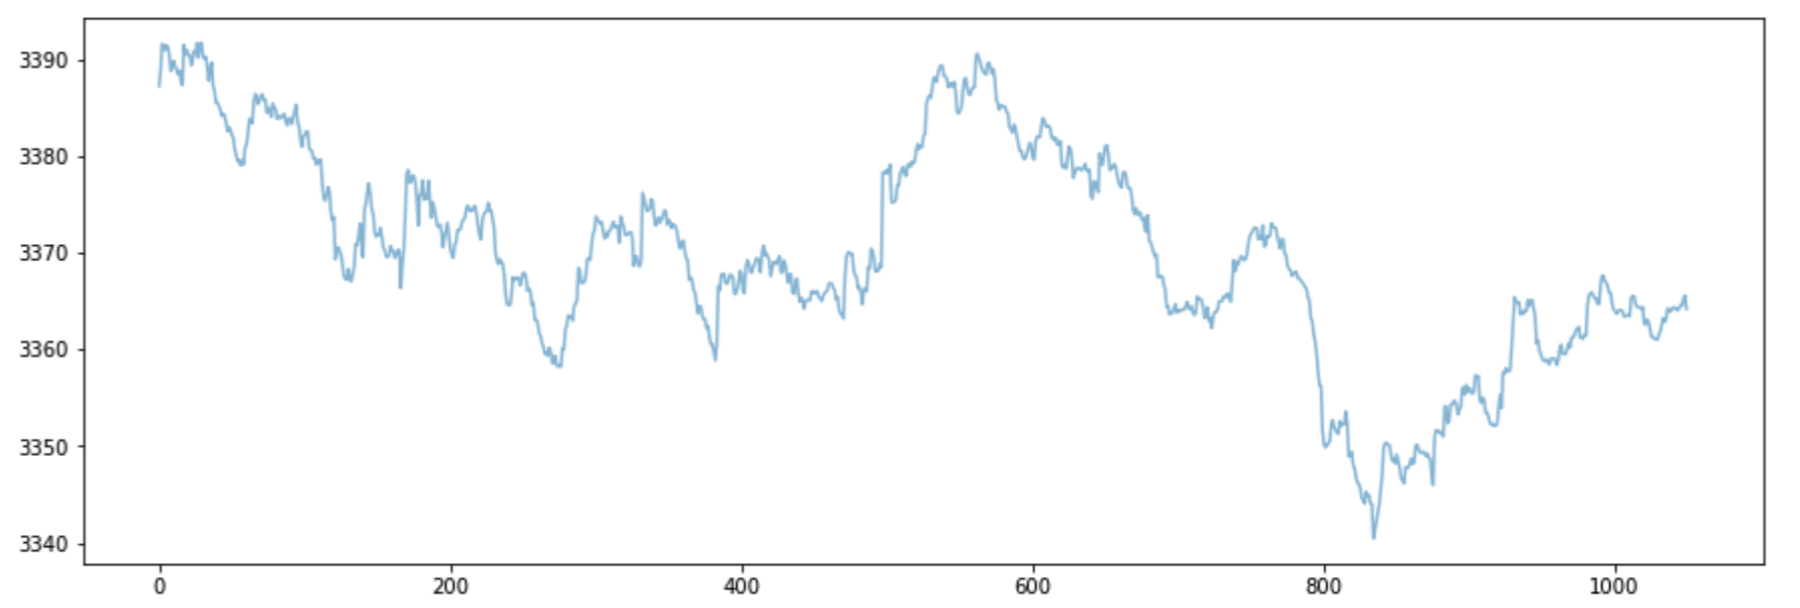
\includegraphics[width=1\textwidth]{../paper/images/stock_example.png}
            \caption{An Example of Stock Price Fluctuations Over Time (Time (s) vs Price)}
            \label{fig:stock}
        \end{center}
    \end{figure}
    
    
    
\end{frame}



%%%%%%%%%%%%%%%%%%%%%%%%%%%%%%%%%%%%%%%%%%%%
%%%%%%%%%%%%%%%%%%%%%%%%%%%%%%%%%%%%%%%%%%%%

\begin{frame}[fragile]{Buy and Sell Advice Based on Breakout Patterns of EMA 38 and 100  }


    \begin{figure}
        \begin{center}
            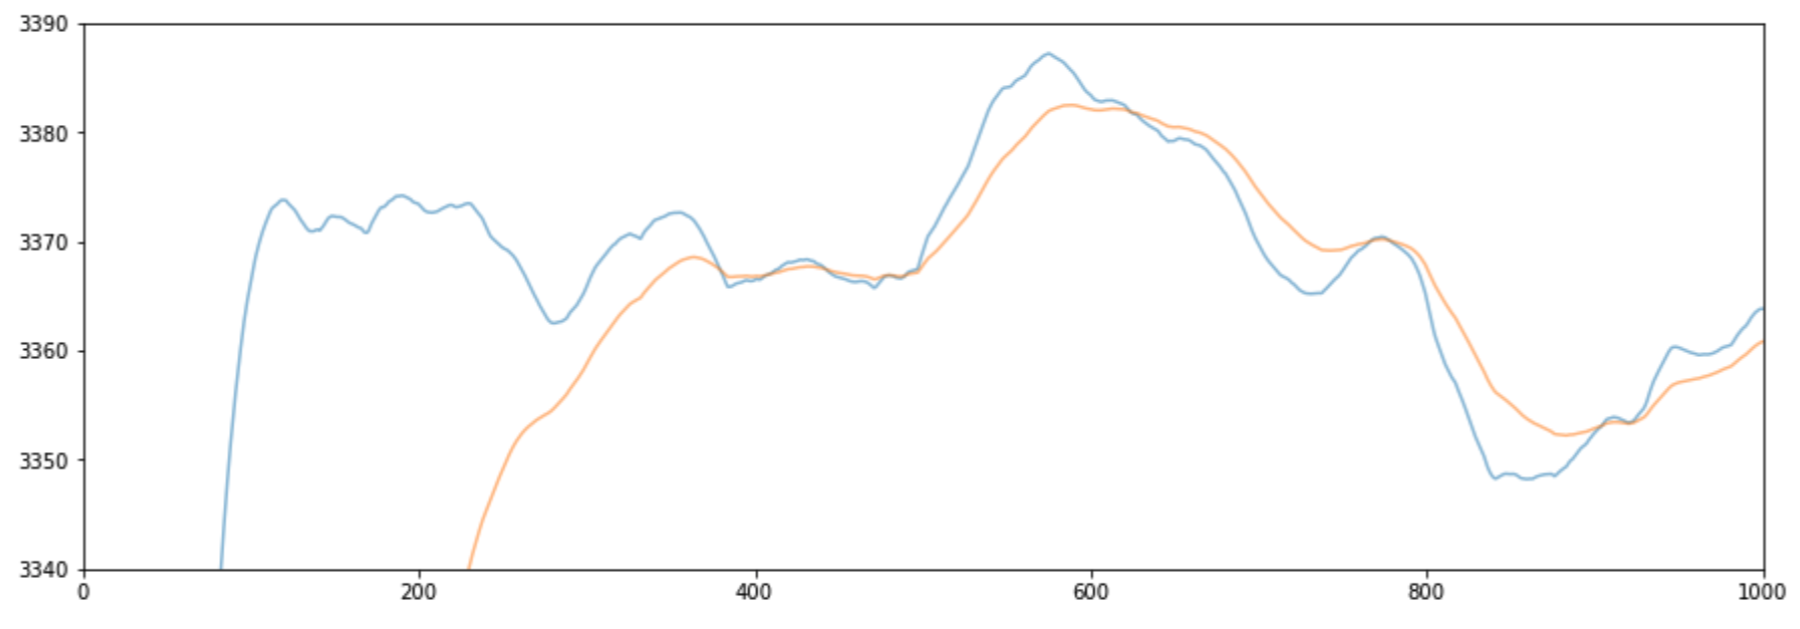
\includegraphics[width=1\textwidth]{../paper/images/query2_example.png}
            \caption{Example of Query 2 (Time (s) vs Price) - Buy and Sell advice based on Breakout Patterns of EMA 38 (orange) and 100 (blue)}
            \label{fig:EMAs}
         \end{center}
    \end{figure}
    
\end{frame}

%%%%%%%%%%%%%%%%%%%%%%%%%%%%%%%%%%%%%%%%%%%%
%%%%%%%%%%%%%%%%%%%%%%%%%%%%%%%%%%%%%%%%%%%%

\begin{frame}[fragile]{ Use one of the OSS or implement from scratch?}


    Should we use one of the Open Source Stream processing systems like: 
\begin{itemize}
    \item \blueb{Apache Spark - Streaming}
    \item \blueb{Apache Flink - Streaming}
    \item \blueb{Apache Storm}
    \item \blueb{Apache Kafka for streaming pipelines} 
    \item \blueb{Esper Stream processing}
    \item \blueb{WindFlow}\footnote{WindFlow data stream processing \url{https://paragroup.github.io/WindFlow/}} in C++ 
    \item  ... 
\end{itemize}

    We decided to implement the DEBS Grand Challenge from scratch. 
    
    \redb{Why?}   
        
\end{frame}


%%%%%%%%%%%%%%%%%%%%%%%%%%%%%%%%%%%%%%%%%%%%
%%%%%%%%%%%%%%%%%%%%%%%%%%%%%%%%%%%%%%%%%%%%

\begin{frame}[fragile]{Why implementing from scratch? }


    \begin{itemize}
            
        \item The Challenge queries are simple, therefore we can optimize the processing in our implementation much better. 
        \item Our stream throughput is not very high. Maximum a Batch of 10k events, as defined by the Challenge. 
        

        \item Systems like Spark or Flink include internal data processes; to name a few: 
        
        \begin{itemize}
            \item Communications between the master and worker processes
            \item Internal caching and pipeline generations including batch processing, blocking data exchanges,
            \item Checkpoint barriers, watermarks signaling or iteration barriers to provide guarantee of a FIFO order of and 
            snapshots of the data stream
   
        \end{itemize}
         
         %  \item Most of these systems are designed in a distributed cluster computing setting which includes cluster managements like communications between the master process/es and worker processes.
        %  Many processes are started as JobManager and TaskManager to coordinate different task executions. 
     
        %  \item These systems are designed to optimize the trade-off between higher scalability and higher stream throughput/latency performance. 
        %  The described DEBS 2022 challenge does not include a very large data stream that we would need to design a high-scalable data stream processing system. 
        %  But our main system design goal is to achieve high throughput and low-latency. 
        %  Systems like Spark or Flink include internal data processing pipelines including batch processing and blocking data exchanges. 
    
        \item Lots of configuration parameters which modify the performance/latency. 
        
        % These systems are designed to optimize the trade-off between higher scalability and higher stream throughput/latency performance. 
        % The described DEBS 2022 challenge does not include a very large data stream that we would need to design a high-scalable data stream processing system. 
        % But our main system design goal is to achieve high throughput and low-latency. 
        % Systems like Spark or Flink include internal data processing pipelines including batch processing and blocking data exchanges. 
        
        % \item 
        
        % Such systems use special types of control events, like  checkpoint barriers, watermarks signaling or iteration barriers to provide guarantee of a FIFO order of
        %  events, to generate snapshots of the data stream for example, or be able to do stream recovery \cite{df177547a4364bb0a7e2470b83025bb0}. 
        % In our system we can make sure that our stream processing is a stateful processing, and windows are correctly generated from the stream batches. 
        % And no additional internal batch generations are needed. 
    
        % \item 
        
        % The cluster stream processing systems have many configuration parameters which modify the performance stream processing. 
        % For example, the configuration parameters control the number of cluster executor processes and threads. 
        % With our implementation, we can better control the system parameters like number of processes or threads. 

    
    \end{itemize}

    \redb{Our goal was correctness with highest possible throughput and low latency.} 

    
\end{frame}


%%%%%%%%%%%%%%%%%%%%%%%%%%%%%%%%%%%%%%%%%%%%
%%%%%%%%%%%%%%%%%%%%%%%%%%%%%%%%%%%%%%%%%%%%

\section{Architectural Design}

%%%%%%%%%%%%%%%%%%%%%%%%%%%%%%%%%%%%%%%%%%%%
%%%%%%%%%%%%%%%%%%%%%%%%%%%%%%%%%%%%%%%%%%%%

\begin{frame}[fragile]{Parallel Processing }


    \begin{figure}[ht]
        \begin{center}
            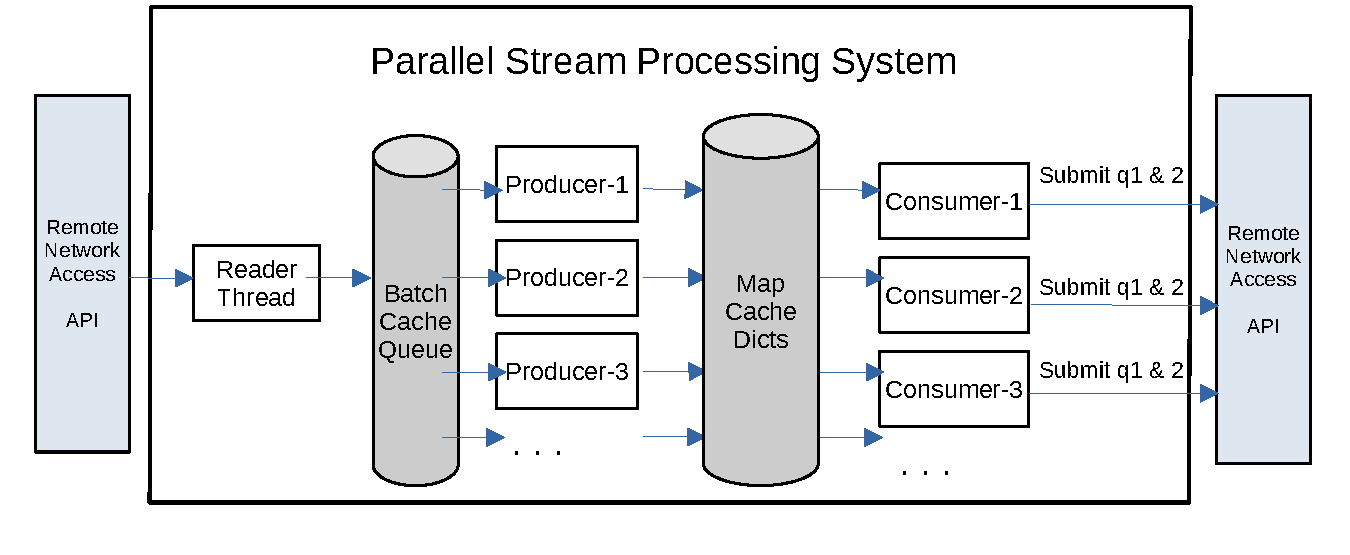
\includegraphics[width=0.8\textwidth]{../paper/images/Parallel-Stream-Processing-System_v2}
            \caption{Parallel Processing of Events By a Set of Producers and Consumers without a Data Dispatcher.}
            \label{fig:parallel-srream-processing1}
        \end{center}
    \end{figure}

    \begin{itemize}
        \item Reading Batches and Caching them 
        \item The Reader reads from the DEBS Challenge API
        \item The Submitter had to be a single submitter
    \end{itemize}

    
\end{frame}




%%%%%%%%%%%%%%%%%%%%%%%%%%%%%%%%%%%%%%%%%%%%
%%%%%%%%%%%%%%%%%%%%%%%%%%%%%%%%%%%%%%%%%%%%

\begin{frame}[fragile]{Event Dispatcher and Submitter Architecture }
    
    \begin{figure}[h]
        \begin{center}
            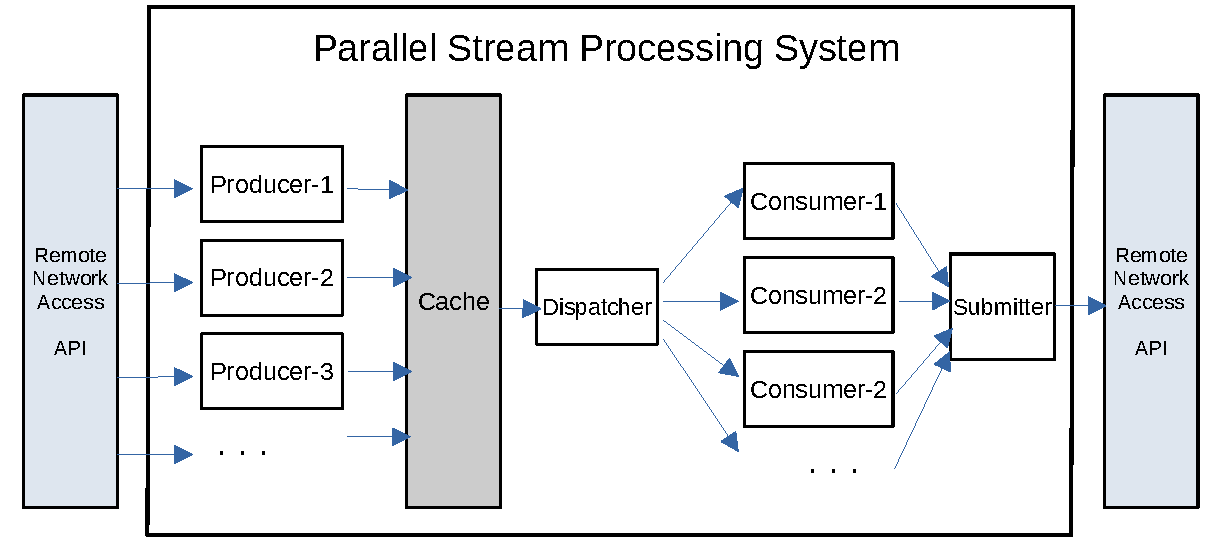
\includegraphics[width=0.8\textwidth]{../paper/images/Parallel-Stream-Processing-System}
            \caption{Event Dispatcher and Submitter Architecture}
            \label{fig:parallel-srream-processing}
        \end{center}
    \end{figure}


    \begin{itemize}
        \item Event Batch Dispatcher distributes the batches
        \item Producers read the Event from API, create internal data windows
        \item Event Windows are cached similar to Figure \ref{fig:parallel-srream-processing1} 
    \end{itemize}
    
\end{frame}



%%%%%%%%%%%%%%%%%%%%%%%%%%%%%%%%%%%%%%%%%%%%
%%%%%%%%%%%%%%%%%%%%%%%%%%%%%%%%%%%%%%%%%%%%

\begin{frame}[fragile]{Event Data Dispatcher  }

        \begin{figure}
            \begin{center}
                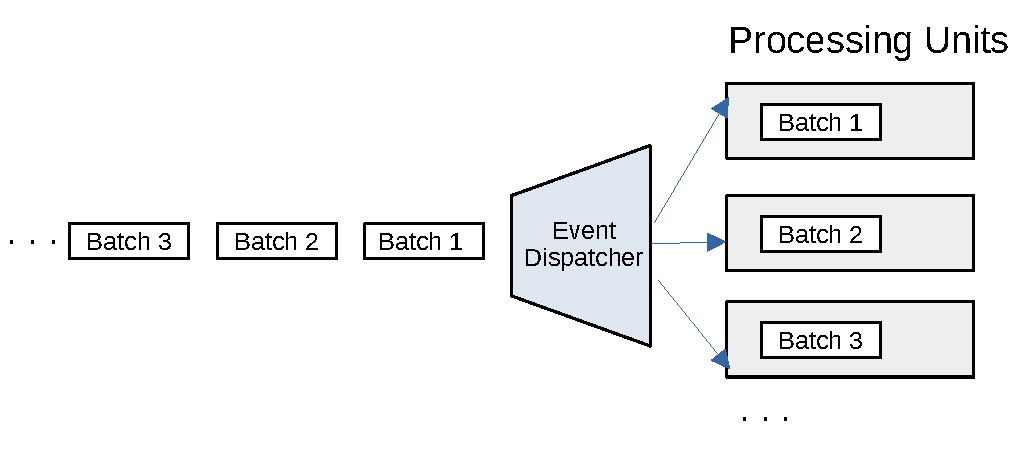
\includegraphics[width=0.7\textwidth]{../paper/images/Stream-Batch-Distributions}
                \caption{An Event Data Dispatcher}
                \label{fig:batch-distributions}
            \end{center}
        \end{figure}
     
        \begin{figure}
            \begin{center}
                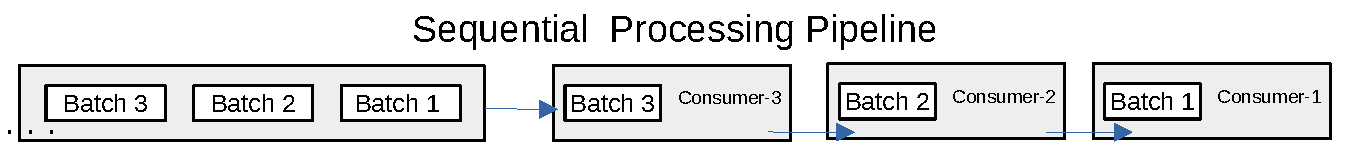
\includegraphics[width=1\textwidth]{../paper/images/Stream-Batch-Distributions_op2}
                \caption{A Sequential Processing Pipeline. Each consumer reads a batch and passes to the next consumer.}
                \label{fig:Sequential-batch-distributions}
            \end{center}
        \end{figure}

\end{frame}








%%%%%%%%%%%%%%%%%%%%%%%%%%%%%%%%%%%%%%%%%%%%
%%%%%%%%%%%%%%%%%%%%%%%%%%%%%%%%%%%%%%%%%%%%

% \begin{frame}[fragile]{ Sequential Processing Pipeline }
    

 
%     \begin{figure}
%         \begin{center}
%             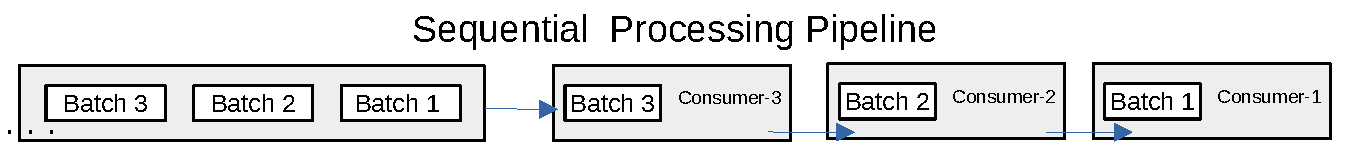
\includegraphics[width=1\textwidth]{../paper/images/Stream-Batch-Distributions_op2}
%             \caption{A Sequential Processing Pipeline. Each consumer reads a batch and passes to the next consumer.}
%             \label{fig:Sequential-batch-distributions}
%         \end{center}
%     \end{figure}


% \end{frame}





% %%%%%%%%%%%%%%%%%%%%%%%%%%%%%%%%%%%%%%%%%%%%
% %%%%%%%%%%%%%%%%%%%%%%%%%%%%%%%%%%%%%%%%%%%%

% \begin{frame}[fragile]{Parallel Processing with an Event Data Dispatcher  }

%     \begin{figure}
%         \begin{center}
%             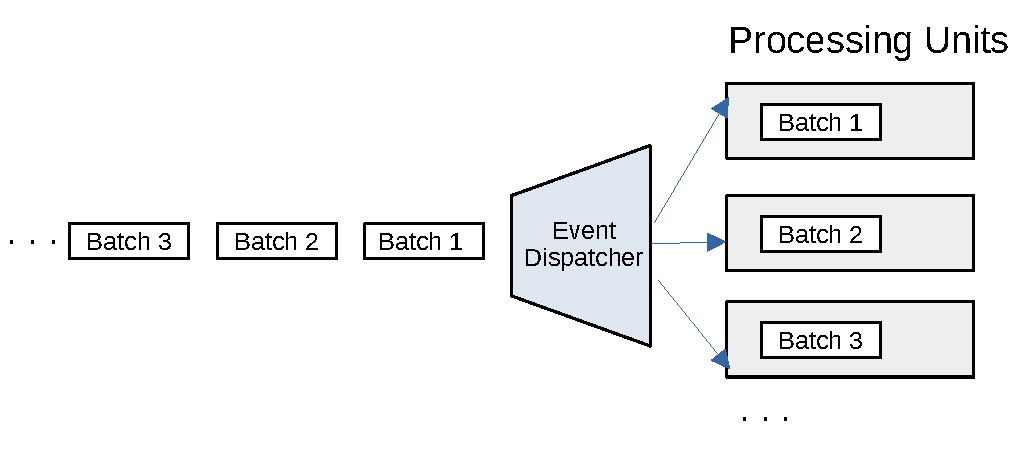
\includegraphics[width=0.7\textwidth]{../paper/images/Stream-Batch-Distributions}
%             \caption{An Event Data Dispatcher}
%             \label{fig:batch-distributions}
%         \end{center}
%     \end{figure}

% \end{frame}




%%%%%%%%%%%%%%%%%%%%%%%%%%%%%%%%%%%%%%%%%%%%
%%%%%%%%%%%%%%%%%%%%%%%%%%%%%%%%%%%%%%%%%%%%


\section{Implementation}



%%%%%%%%%%%%%%%%%%%%%%%%%%%%%%%%%%%%%%%%%%%%
%%%%%%%%%%%%%%%%%%%%%%%%%%%%%%%%%%%%%%%%%%%%

\begin{frame}[fragile,t ]{Two Implementations in Python and Java }
    \begin{itemize}
        \item  Source Code is available here \url{https://github.com/kiat/debs2022/}
  
    \end{itemize}
   \vspace*{1cm}


    Two Implementations in Python and Java:
    \begin{itemize}
        \item Our first implementation was a multi-threaded Python 
        % to make sure we can process the queries in the correct form.
        \item We have done a subsequent implementation in Java.  
    \end{itemize}

    % Our first rapid alpha implementation of the system was a multi-threaded Python implementation to make sure that we understood the challenge tasks and are able to process the queries in the correct form.
    % Later, we implemented the whole system again in Java. Both of these implementations are open sourced on Github\footnote{\url{https://github.com/kiat/debs2022} , last update June, 2022}.
    
    % Our Java implementation includes two simple threads, one is the event producer (or event batch Reader Thread that communicates over the DEBS Challenge API). 
    % The Reader reads the stream of event batches, creates and adds event batch windows (5 min. windows) to an intermediate cache. In parallel, another consumer thread processes the cached event windows data 
    % for the results of query 1 and query 2. We have integrated processing the query 2 with the Query 1 task within the consumer thread. 
    % The caches are java lists of batches and a java HashMap that caches event windows for each stock symbols. 
    % To achieve better performance we pre-allocate both of these caches Java ArrayList and HashMap with a specific size. 
    % The two threads are synchronized over a simple lock mechanism and thread notification. The results of both queries are submitted by the consumer thread to the DEBS Challenge API.
    
    
\end{frame}


%%%%%%%%%%%%%%%%%%%%%%%%%%%%%%%%%%%%%%%%%%%%
%%%%%%%%%%%%%%%%%%%%%%%%%%%%%%%%%%%%%%%%%%%%

\begin{frame}[fragile]{ Python Implementation }

    % ADD YOUR IDEAS HERE

    Summary of the Python implementation:
    
    \begin{itemize}
        \item Our first, alpha prototype
        \item Assured correctness of Query Processing 
        \item Allowed for an implementation that could quickly be built
        \item Included multithreading, giving a baseline for experiments
        \item Provided context for further improvements, i.e. a Java implementation

    \end{itemize}


    
\end{frame}

%%%%%%%%%%%%%%%%%%%%%%%%%%%%%%%%%%%%%%%%%%%%
%%%%%%%%%%%%%%%%%%%%%%%%%%%%%%%%%%%%%%%%%%%%

\begin{frame}[fragile]{Our Java implementation }
    
    Our Java implementation includes two simple threads, one is the event producer (or event batch Reader Thread that communicates over the DEBS Challenge API), and the other is a submitter, that processes cached event windows data for queries 1 and 2. 
    \begin{itemize}
        \item Two simple threads:
        \begin{itemize}
            \item Event producer for main query computations
            \item Result submitter
        \end{itemize}
        % one is the event producer and one is the main query processor,  and result submitter. 
        \item We use a Java lists of batches, and a Java HashMap to cache event windows for each stock symbols. 
        \item Pre-allocate both of these caches in Java ArrayList and HashMap with a specific size.
        \item Threads are synchronized over a lock mechanism and thread notification.
        \item The results of both queries are submitted by the consumer thread to the DEBS Challenge API.
        \item With Batch Size 10k, two Threads was enough. 
    \end{itemize}


    
\end{frame}




%%%%%%%%%%%%%%%%%%%%%%%%%%%%%%%%%%%%%%%%%%%%
%%%%%%%%%%%%%%%%%%%%%%%%%%%%%%%%%%%%%%%%%%%%

\section{Experiments}





%%%%%%%%%%%%%%%%%%%%%%%%%%%%%%%%%%%%%%%%%%%%
%%%%%%%%%%%%%%%%%%%%%%%%%%%%%%%%%%%%%%%%%%%%

\begin{frame}[fragile]{Python with Batch Size 1K  }
    
    \begin{figure}
        \begin{center}
            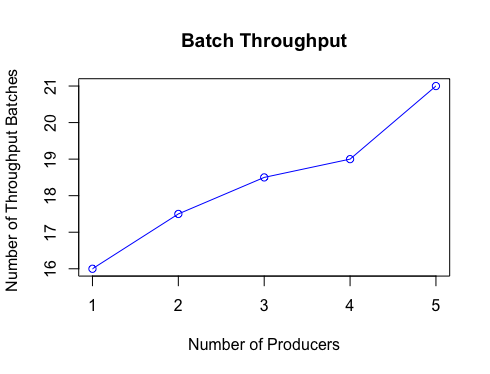
\includegraphics[width=0.7\textwidth]{../paper/images/throughput.png}
            \caption{Query 2 throughput for different number of Producers. (Batch Size 1k - Multi-threaded Python implementation) }
            \label{fig:evaluation}
        \end{center}
    \end{figure}
\end{frame}






%%%%%%%%%%%%%%%%%%%%%%%%%%%%%%%%%%%%%%%%%%%%
%%%%%%%%%%%%%%%%%%%%%%%%%%%%%%%%%%%%%%%%%%%%

\begin{frame}[fragile]{Java with Batch Size 10K  }
    \begin{itemize}
        \item Our Java implementation has higher performance because of some language features (Like static variable types and improved iterations over event batches).
        \item Latency of 19.99 seconds and a 88.21 batches per seconds
    \end{itemize}

    
    % According to the DEBS 2022 evaluation \cite{debs2022challenge} server, our Java implementation can achieve a latency of 19.99 seconds and a 88.21 batch per 
    % seconds with an event batch size of 10k (events arriving in batches of 10k).

    
    \begin{figure}[]
        \begin{center}
            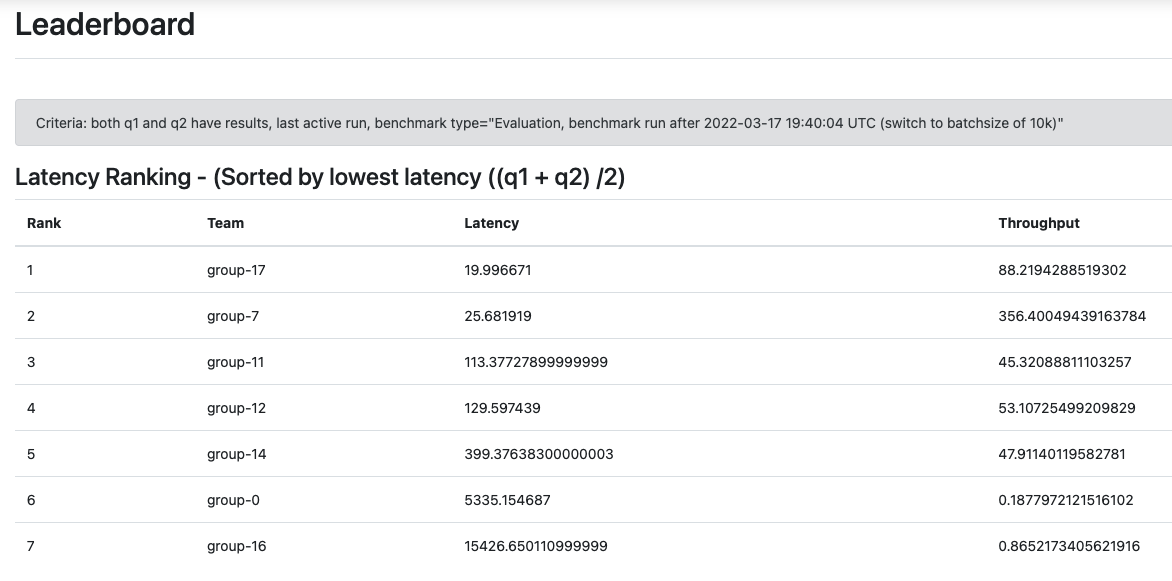
\includegraphics[width=0.8\textwidth]{../DEBS2022-2022-05-28-Throuput.png}
            \caption{Our group, Group 17, Results }
            \label{fig:evaluation}
        \end{center}
    \end{figure}
    
\end{frame}



%%%%%%%%%%%%%%%%%%%%%%%%%%%%%%%%%%%%%%%%%%%%
%%%%%%%%%%%%%%%%%%%%%%%%%%%%%%%%%%%%%%%%%%%%


\section{Conclusion}

%%%%%%%%%%%%%%%%%%%%%%%%%%%%%%%%%%%%%%%%%%%%
%%%%%%%%%%%%%%%%%%%%%%%%%%%%%%%%%%%%%%%%%%%%



%%%%%%%%%%%%%%%%%%%%%%%%%%%%%%%%%%%%%%%%%%%%
%%%%%%%%%%%%%%%%%%%%%%%%%%%%%%%%%%%%%%%%%%%%

\begin{frame}[fragile]{Conclusion and Future Work}
    \begin{itemize}
        \item Our implementation and evaluation are limited due to the time constraints we had for this work.
        
        \item We observed how our from-scratch-implemented system performed compared to some large-scale cluster-based stream processing systems like Apache Storm or Flink (implemented by other groups).
        
        \item One potential improvement would be to implement it using a system programming language like C++ or Rust.
        
        \item This solution has scalability potential, from larger batch sizes, to more threads, to parallel computing. 
    \end{itemize}

    
    

\end{frame}




% %%%%%%%%%%%%%%%%%%%%%%%%%%%%%%%%%%%%%%%%%%%%
% %%%%%%%%%%%%%%%%%%%%%%%%%%%%%%%%%%%%%%%%%%%%

% \begin{frame}[fragile]{  }
    

% \end{frame}

\end{document}